\documentclass[12pt]{article}
\usepackage{fontspec}
\usepackage{polyglossia}
\setmonofont{Courier New}
\setmainlanguage{farsi}
\setotherlanguage{english}
\newfontfamily\persianfont[Script=Arabic]{XBZar}
\usepackage{graphicx}
\usepackage{geometry}
\usepackage{hyperref}
\geometry{a4paper, margin=2.5cm}
\usepackage{setspace}
\usepackage{url}
\onehalfspacing
\usepackage{titling}
\usepackage{float}
\usepackage{etoolbox}
\usepackage[backend=biber,style=numeric,sorting=none]{biblatex}
%%%%%%%%%%%%%%%%%%%%%%%%%%%%%%%%%%%%%%%%%%%%%%%%%%%%%%%%%%%%%%%%%%%%%%%%%%%%%
\makeatletter
\newcommand{\persiandigit}[1]{%
	\ifcase#1 ۰\or ۱\or ۲\or ۳\or ۴\or ۵\or ۶\or ۷\or ۸\or ۹\fi
}
\DeclareFieldFormat{labelnumber}{\persiandigit{#1}}
\makeatother
%%%%%%%%%%%%%%%%%%%%%%%%%%%%%%%%%
\newcommand{\persianordinal}[1]{%
	\ifcase#1
	\or اول%
	\or دوم%
	\or سوم%
	\or چهارم%
	\or پنجم%
	\or ششم%
	\or هفتم%
	\or هشتم%
	\or نهم%
	\or دهم%
	\or یازدهم%
	\or دوازدهم%
	\or سیزدهم%
	\or چهاردهم%
	\or پانزدهم%
	\or شانزدهم%
	\or هفدهم%
	\or هجدهم%
	\or نوزدهم%
	\or بیستم%
	\else #1\fi
}

\newcommand{\persianordinalpage}{\persianfont\persianordinal{\value{page}}}


%%%%%%%%%%%%%%%%%%%%%%%%%%%%%%%%%%%%%%%%%%%%%%%%%%%%%%%%%%%%%%%%%%%%%%%%%%%%%
\begin{filecontents}{\jobname.bib}
	@online{a1,
		url = {https://www.kernel.org/doc/html/latest/admin-guide/sysctl/kernel.html#kernel-parameters}
	}
	@online{a2,
		url = {https://unix.stackexchange.com/questions/333225/which-process-is-proc-self-for}
	}
	
\end{filecontents}

\addbibresource{\jobname.bib}

\defbibheading{bibliography}[]{%
	\begin{RTL}
		\section*{مراجع}
	\end{RTL}
}

%%%%%%%%%%%%%%%%%%%%%%%%%%%%%%%%%%%%%%%%%%%%%%%%%%%%%%%%%%%%%%%%%%%%%%%%%%%%%

\begin{document}
	
	% ==============================
	% Title Page
	% ==============================
	\begin{titlepage}
		\centering
		\vspace*{1cm}
		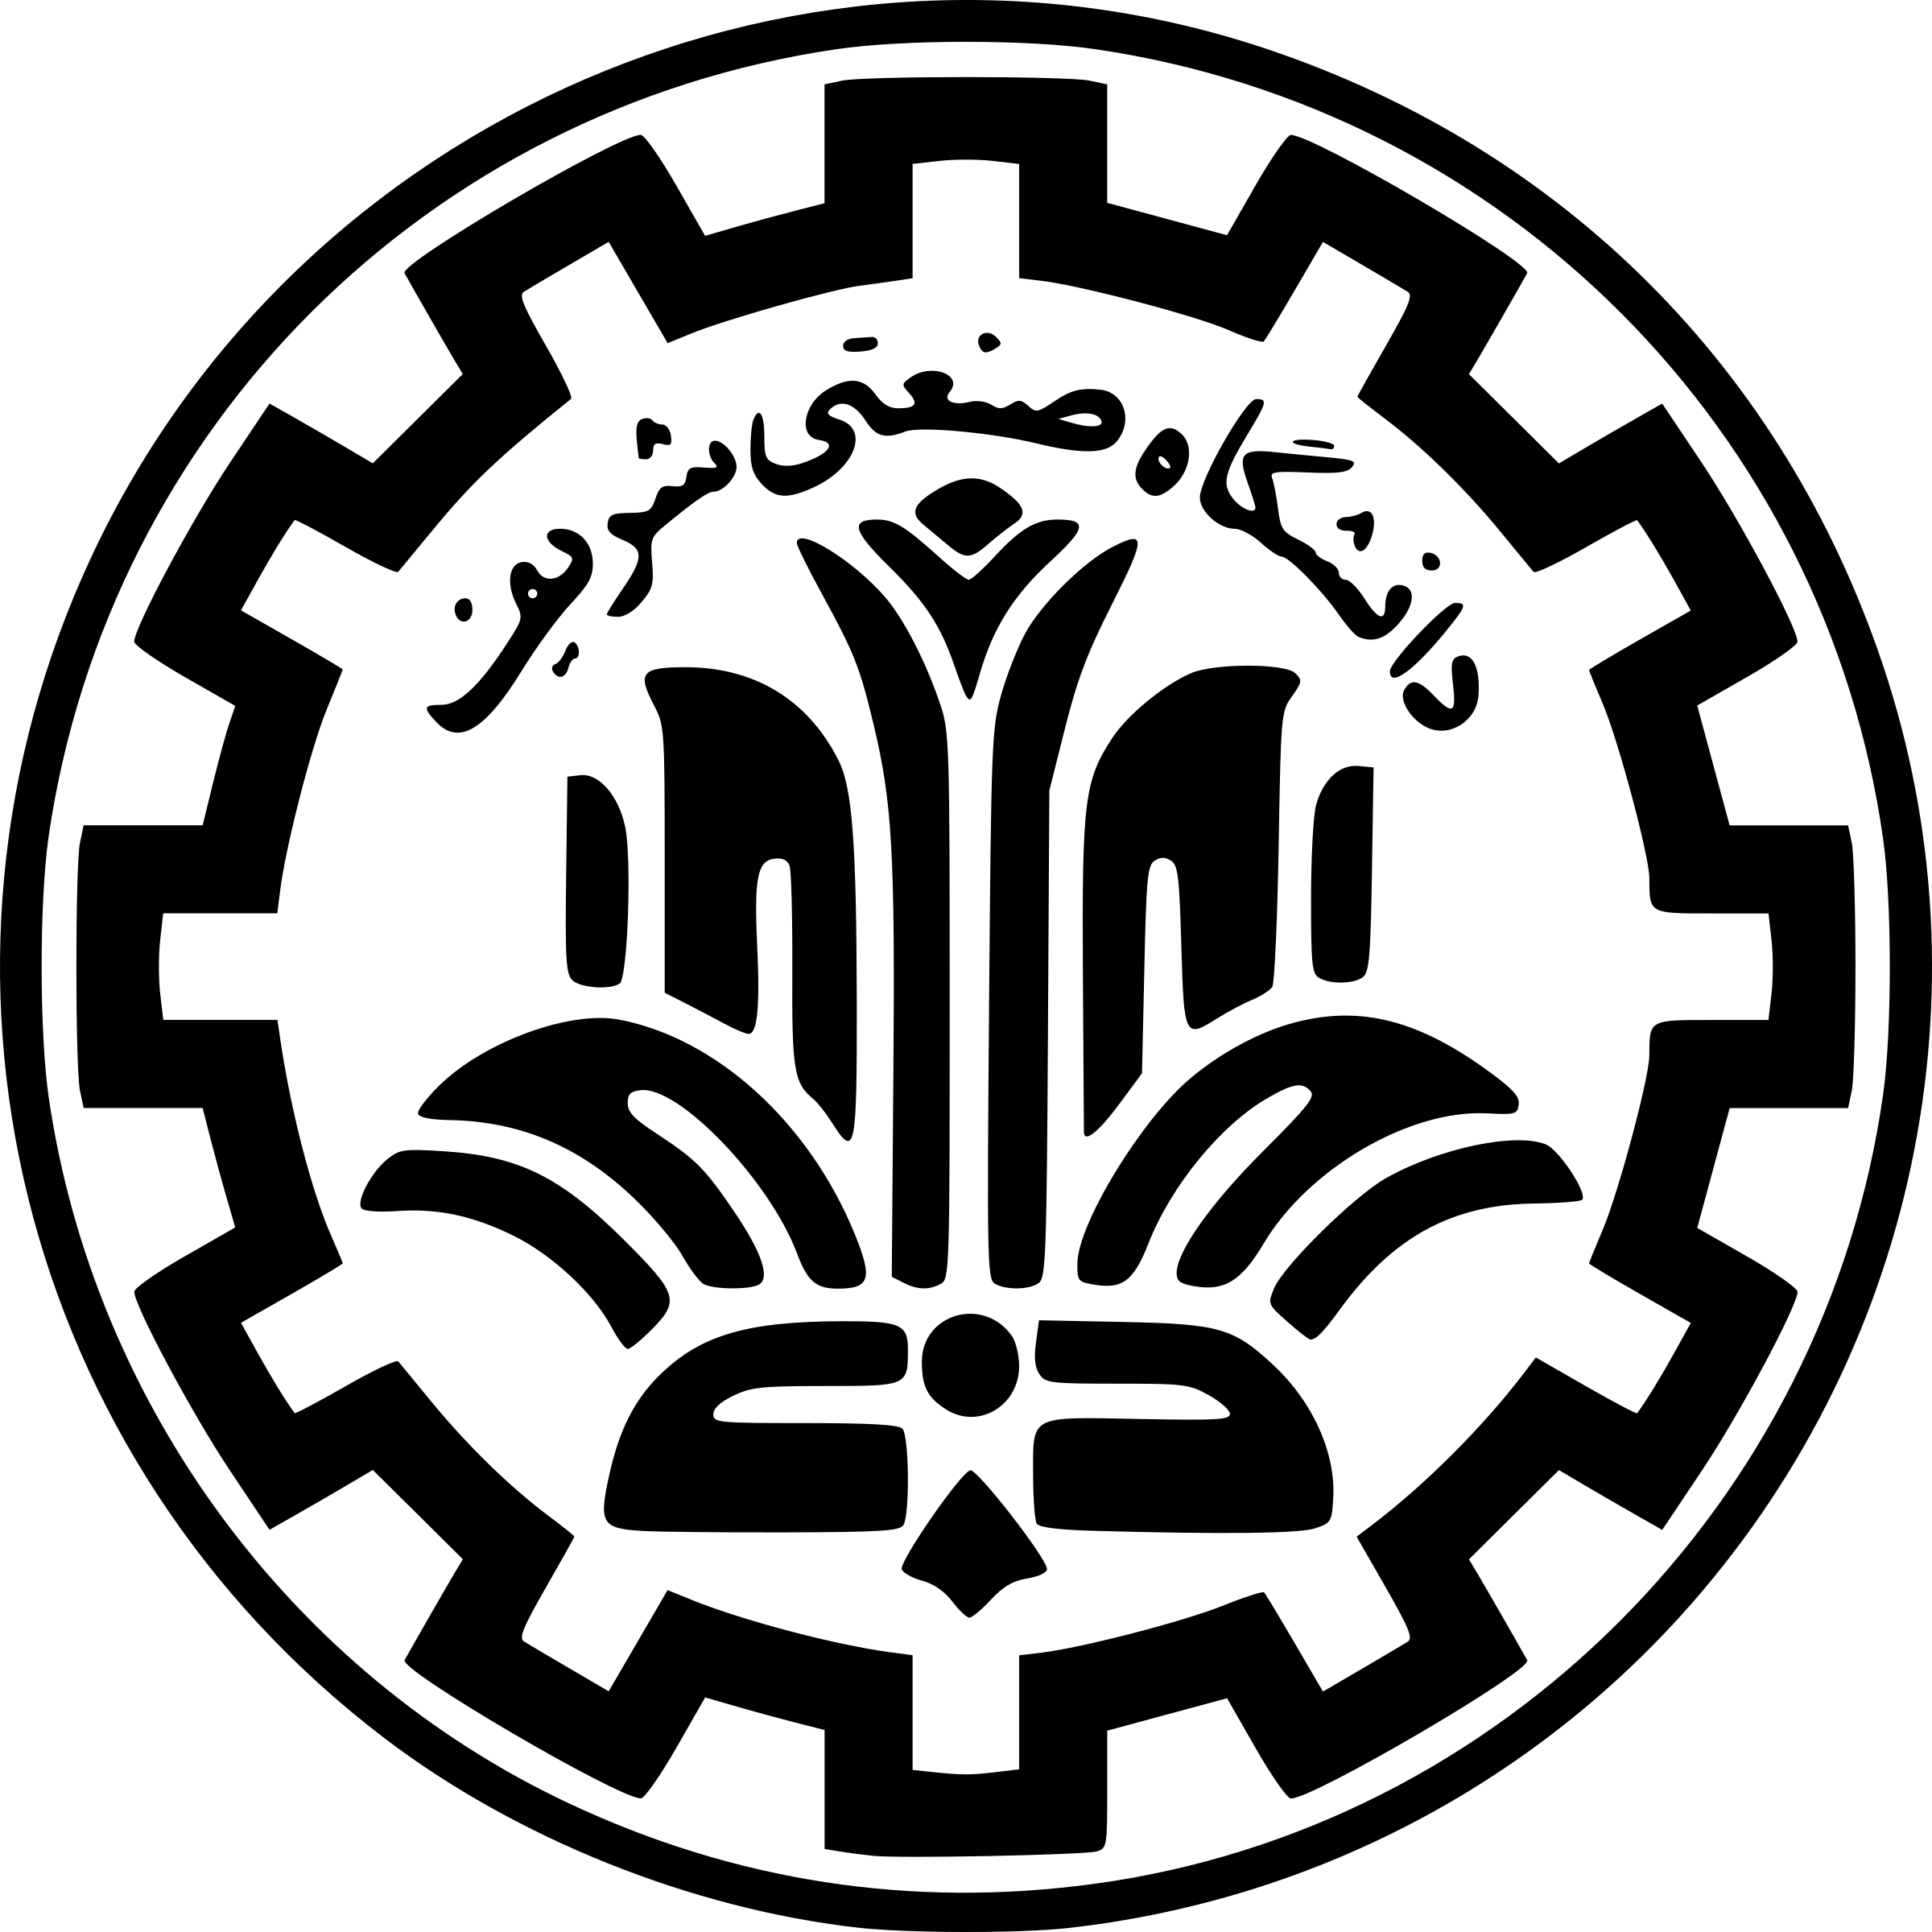
\includegraphics[width=4cm]{sharif.png}\\[1.5cm]
		{\Large\textbf{دانشگاه صنعتی شریف}}\\[0.5cm]
		{\large\textbf{دانشکدهٔ مهندسی کامپیوتر}}\\[1.5cm]
		{\Huge\textbf{گزارش کار آزمایشگاه}}\\[0.5cm]
		{\LARGE\textbf{آزمایشگاه سیستم‌های عامل}}\\[2cm]
		
		\textbf{گزارش آزمایش شماره ۳}\\
		(مشاهده رفتار هسته و سیستم‌عامل)
		
		\vfill
		\begin{tabular}{rl}
			\textbf{شمارهٔ گروه:} & ۲۰ \\
			\textbf{گروه:} &
			ارشیا یوسف‌نیا (۴۰۱۱۱۰۴۱۵) \\
			& محمدعارف زارع زاده (۴۰۱۱۰۶۰۱۷) \\
			\textbf{استاد درس:} & دکتر بیگی \\
			\textbf{تاریخ:} & تابستان ۱۴۰۴ \\
		\end{tabular}
	\end{titlepage}
	
	% ==============================
	% Persian Ordinal Page Numbering
	% ==============================
	\clearpage
	\setcounter{page}{1}
	\renewcommand{\thepage}{\persianordinalpage}
	
	\tableofcontents
	\clearpage
	\listoffigures
	%\clearpage
	%\listoftables
	
	% ==============================
	% Switch to Persian Digits (۱, ۲, ۳, ...)
	% ==============================
	\clearpage
	\setcounter{page}{1}
	\pagenumbering{arabic}
	\renewcommand{\thepage}{\persianfont\arabic{page}}
	
	
	% ==============================
	% Main Content
	% ==============================
	\section{مشاهده فایل سیستم \textenglish{/proc}}
	در شکل \ref{fig:1} به پوشه گفته‌شده رفتیم و لیستی از فایل‌ها و پوشه‌های داخل آن را دیدیم.
	\begin{figure}[H]
		\centering
		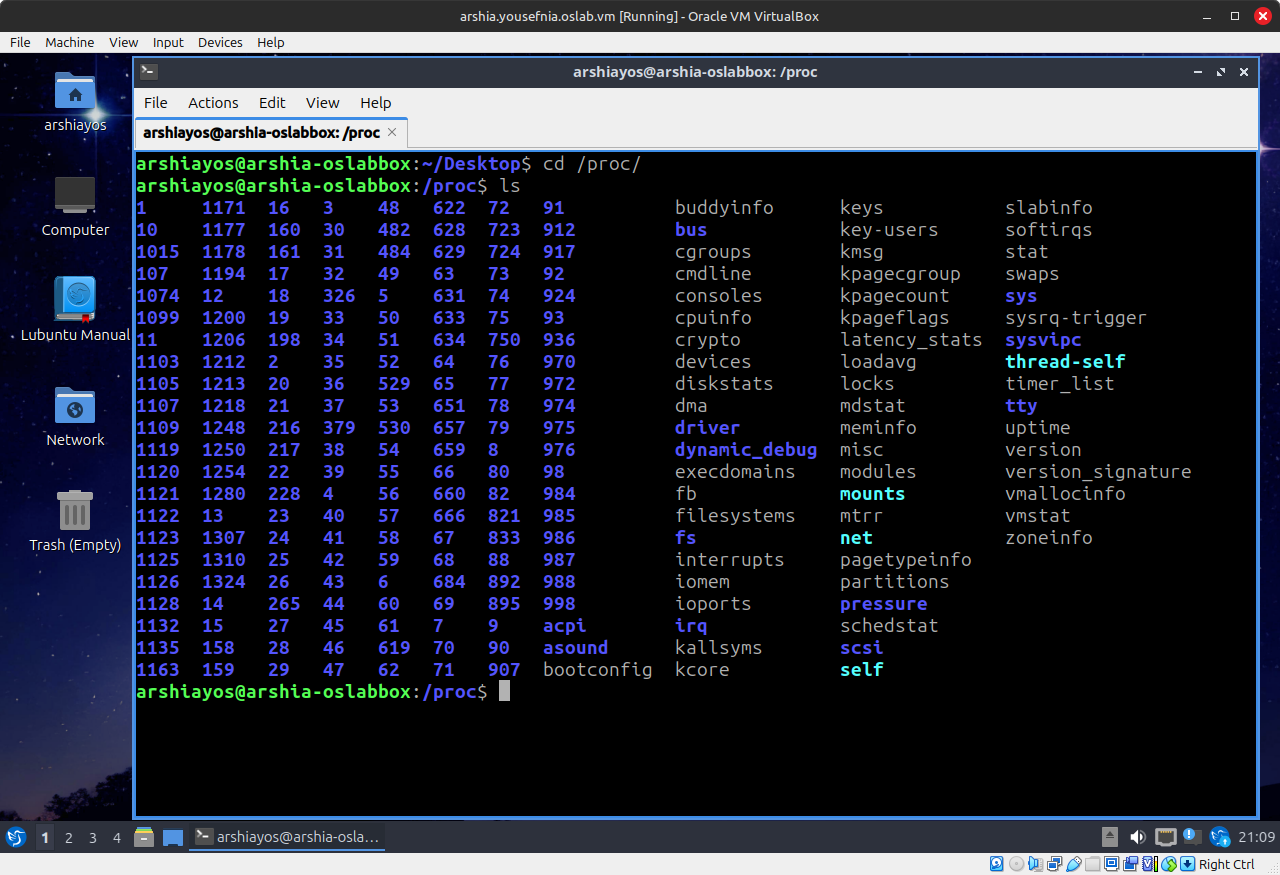
\includegraphics[width=\textwidth]{report3-resources/1.png}
		\caption{محتوای مسیر \textenglish{/proc}}
		\label{fig:1}
	\end{figure}
	
	\newpage
	\section{مشاهده محتویات یک فایل در شاخه \textenglish{/proc}}
	در شکل \ref{fig:2} محتوای فایل version چاپ شده است. همچنین در شکل‌های \ref{fig:3}، 
	\ref{fig:4}،
	\ref{fig:5}، و
	\ref{fig:6}
	هم محتوای بعضی دیگر از فایل‌های این مسیر آمده است. فایل version اطلاعات مربوط به نسخه هسته سیستم‌عامل و دیگر مشخصات آن است. فایل‌های دیگری هم که در شکل‌های بعدی آمده‌اند در بخش آخر این گزارش بیشتر بررسی شده‌اند اما به طور کلی جنبه‌های مختلف سیستم‌عامل از جمله حافظه، فایل‌سیستم‌ها، دستگاه‌های متصل، و موارد دیگر را نشان می‌دهند.
	
	\begin{figure}[H]
		\centering
		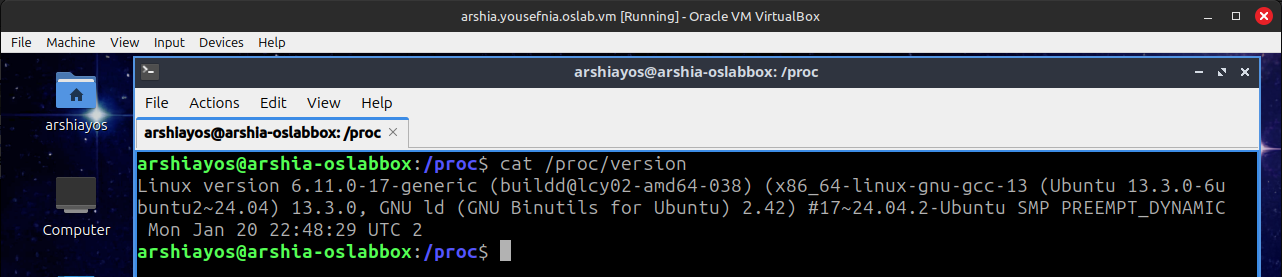
\includegraphics[width=\textwidth]{report3-resources/2.png}
		\caption{چاپ محتوای \textenglish{/proc/version}}
		\label{fig:2}
	\end{figure}
	\begin{figure}[H]
		\centering
		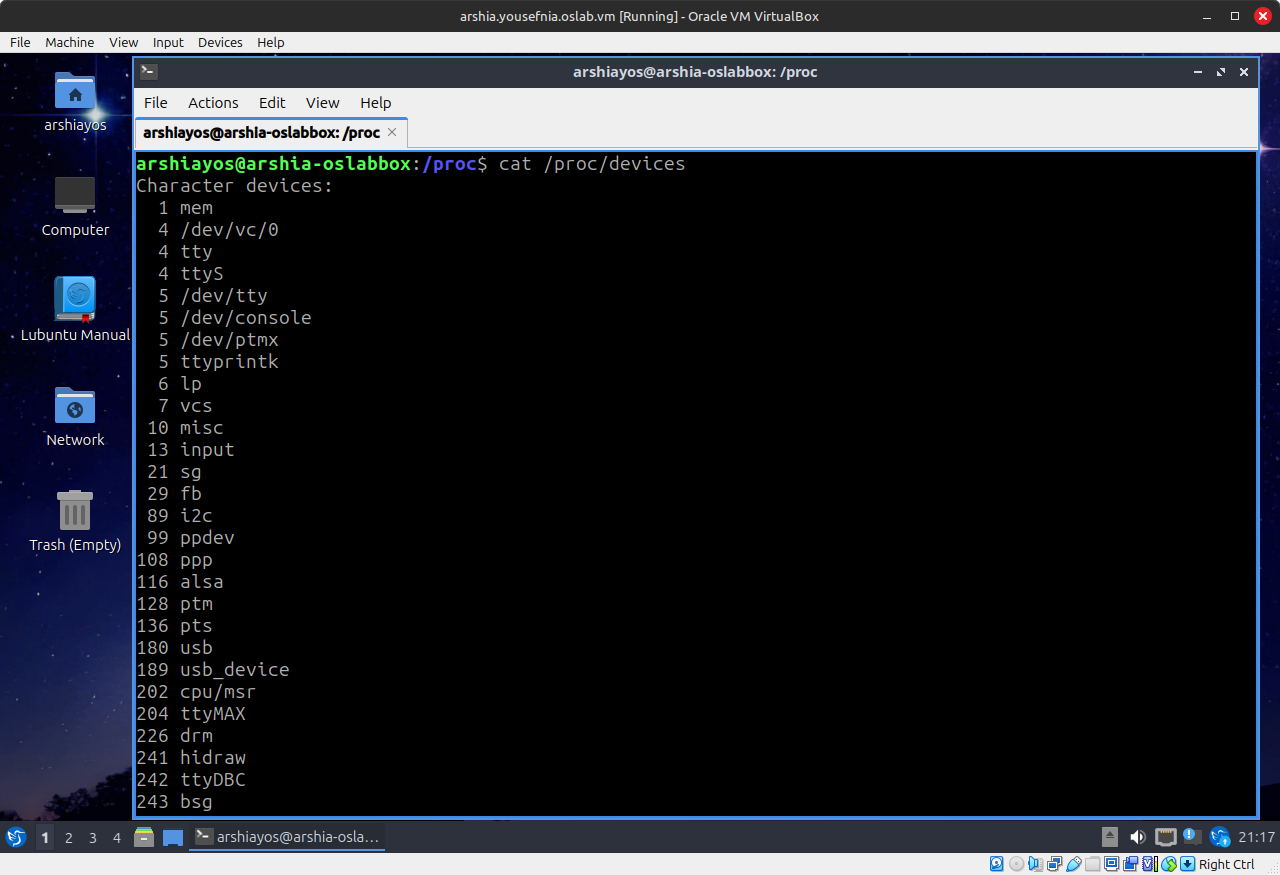
\includegraphics[width=\textwidth]{report3-resources/3.png}
		\caption{چاپ محتوای \textenglish{/proc/devices}}
		\label{fig:3}
	\end{figure}
	\begin{figure}[H]
		\centering
		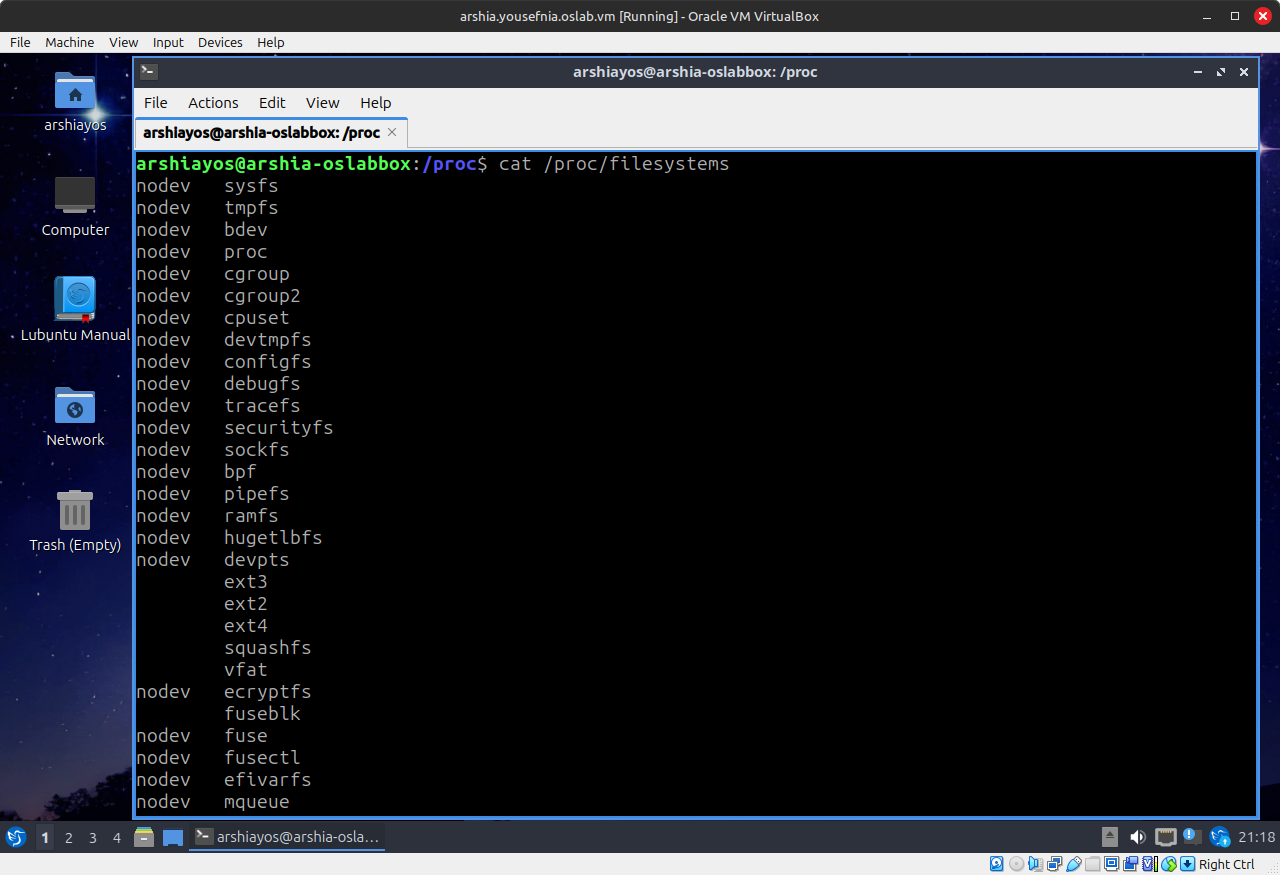
\includegraphics[width=\textwidth]{report3-resources/4.png}
		\caption{چاپ محتوای \textenglish{/proc/filesystems}}
		\label{fig:4}
	\end{figure}
	\begin{figure}[H]
		\centering
		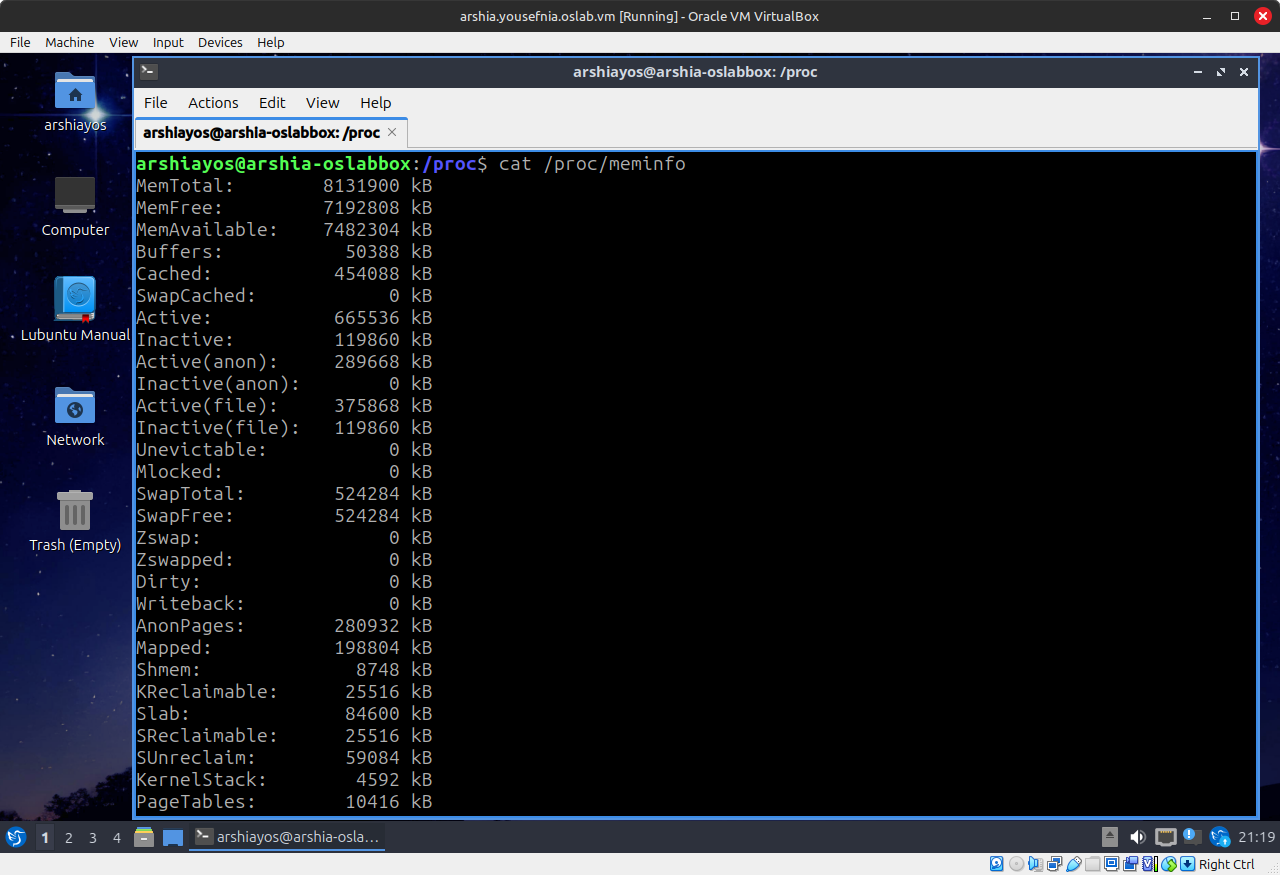
\includegraphics[width=\textwidth]{report3-resources/5.png}
		\caption{چاپ محتوای \textenglish{/proc/meminfo}}
		\label{fig:5}
	\end{figure}
	\begin{figure}[H]
		\centering
		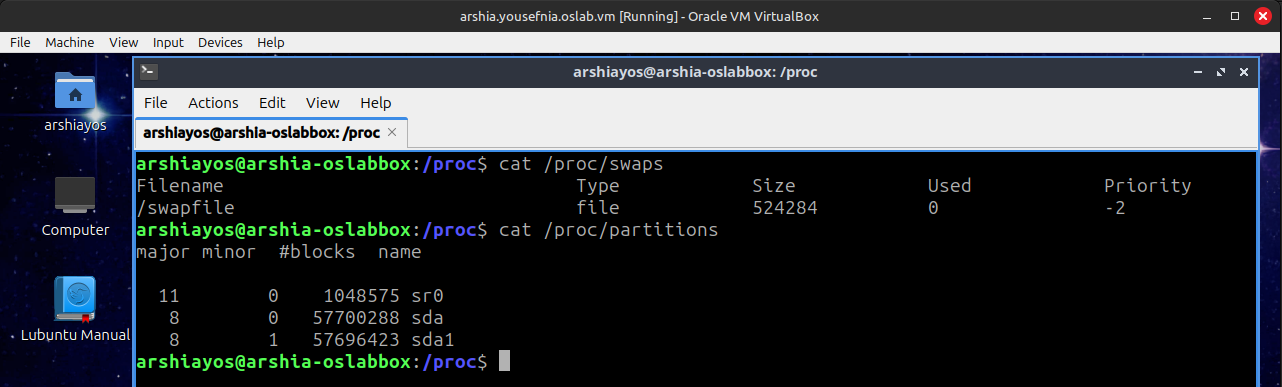
\includegraphics[width=\textwidth]{report3-resources/6.png}
		\caption{چاپ محتوای \textenglish{/proc/swaps, /proc/partitions}}
		\label{fig:6}
	\end{figure}
	در شکل \ref{fig:7} یک برنامه برای خواندن فایل مربوط به نسخه و ریختن آن در فایل دیگر به همراه مراحل کامپایل، اجرا، و نتیجه نهایی آورده‌ایم.
	\begin{figure}[H]
		\centering
		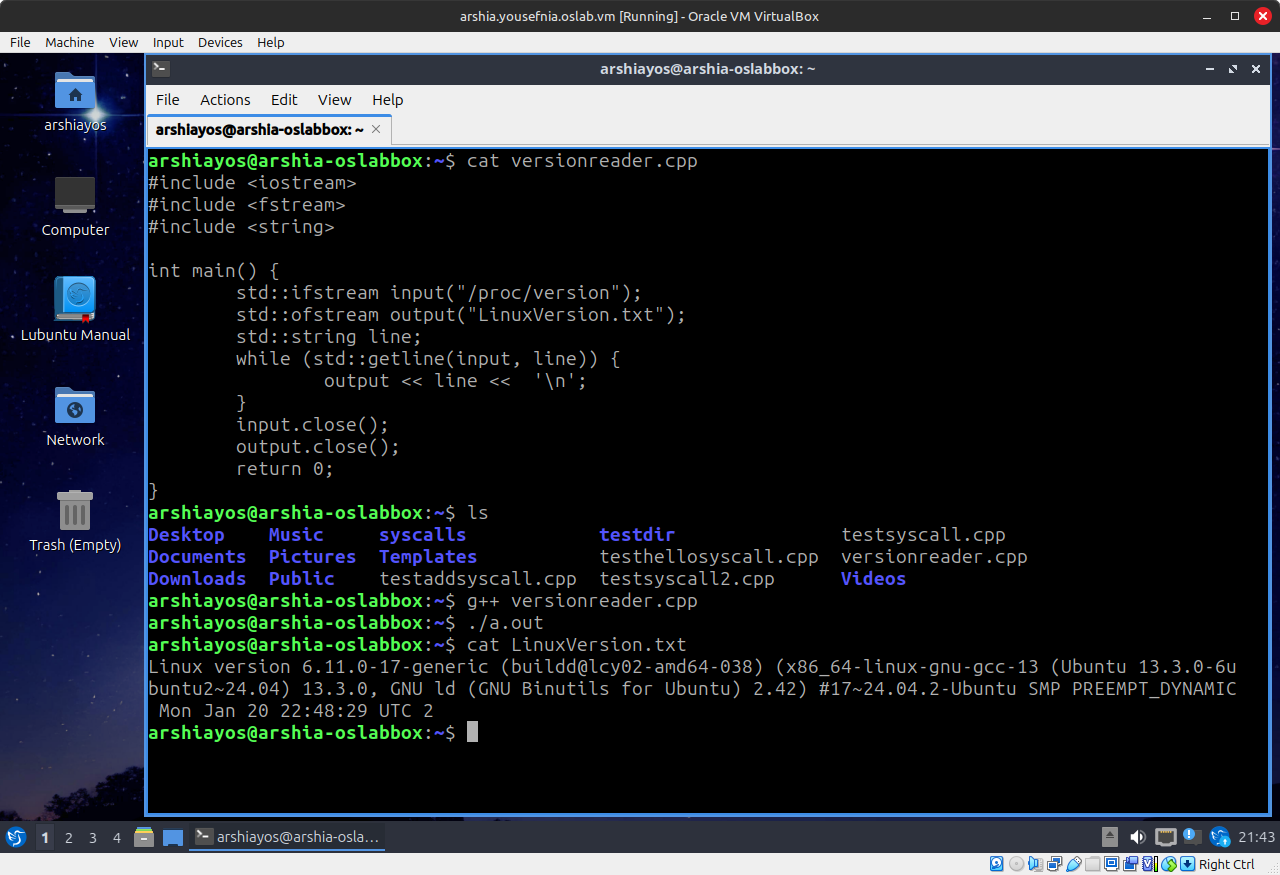
\includegraphics[width=\textwidth]{report3-resources/7.png}
		\caption{یک برنامه cpp برای خواندن محتوای \textenglish{/proc/version} و انتقال آن به فایل \textenglish{LinuxVersion.txt}}
		\label{fig:7}
	\end{figure}
	همانطور که در شکل \ref{fig:8} نشان داده شده امکان نوشتن و تغییر در این فایل‌ها و محتوای در مسیر ویژه /proc نداریم.
	\begin{figure}[H]
		\centering
		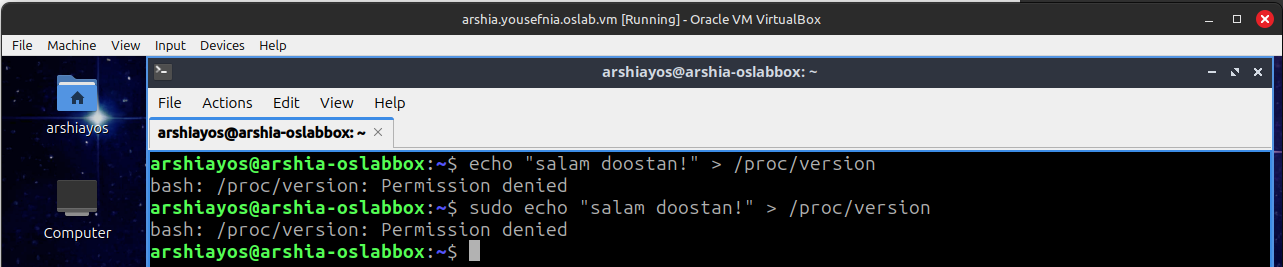
\includegraphics[width=\textwidth]{report3-resources/8.png}
		\caption{نبود دسترسی تغییر در فایل‌های مسیر \textenglish{/proc}}
		\label{fig:8}
	\end{figure}
	
	\newpage
	\section{مشاهده وضعیت پردازه‌ها}
	
	%\begin{figure}[H]
	%	\centering
	%	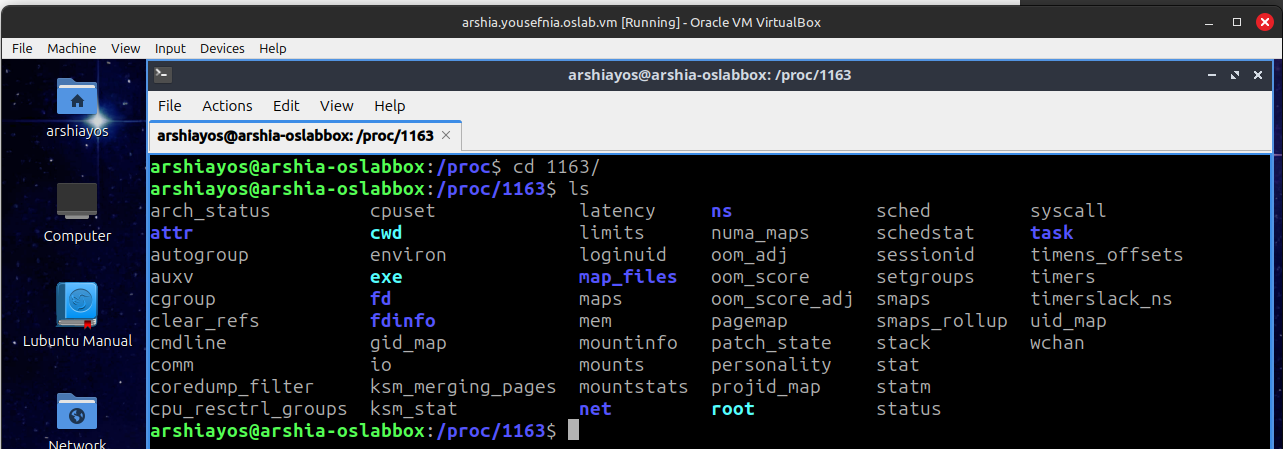
\includegraphics[width=\textwidth]{report3-resources/9.png}
	%	\caption{نمونه‌ای از یک شکل}
	%\end{figure}
	شکل \ref{fig:9} محتوای پوشه یک پردازه را نشان می‌دهد. شکل‌های \ref{fig:10}،
	\ref{fig:11}، و
	\ref{fig:12}
	 به جزییات فایل‌های موجود برای هر پردازه‌ میپردازد.
	 
	 cmdline
	 
	  آرگومان‌های خط فرمان که پردازه با آن اجرا شده است.
	 
	 environ
	 
	  متغیرهای محیطی مربوط به پردازه.

	 stat
	 
	  اطلاعات کلی پردازه مانند PID، وضعیت اجرا، مصرف CPU و غیره.
	 
	 status
	 
	  اطلاعات خلاصه‌شده و قابل‌خواندن درباره وضعیت پردازه.
	 
	 statm
	 
	  اطلاعات حافظه مورد استفاده پردازه (بر حسب صفحات حافظه).
	 
	 cwd
	 
	  لینک به مسیر کاری فعلی پردازه \textenglish{(Current Working Directory)}.
	 
	 exe
	 
	  لینک به فایل اجرایی پردازه.
	 
	 root
	 
	  ریشه مجازی پردازه (برای chroot شده‌ها مفید است).

	\begin{figure}[H]
		\centering
		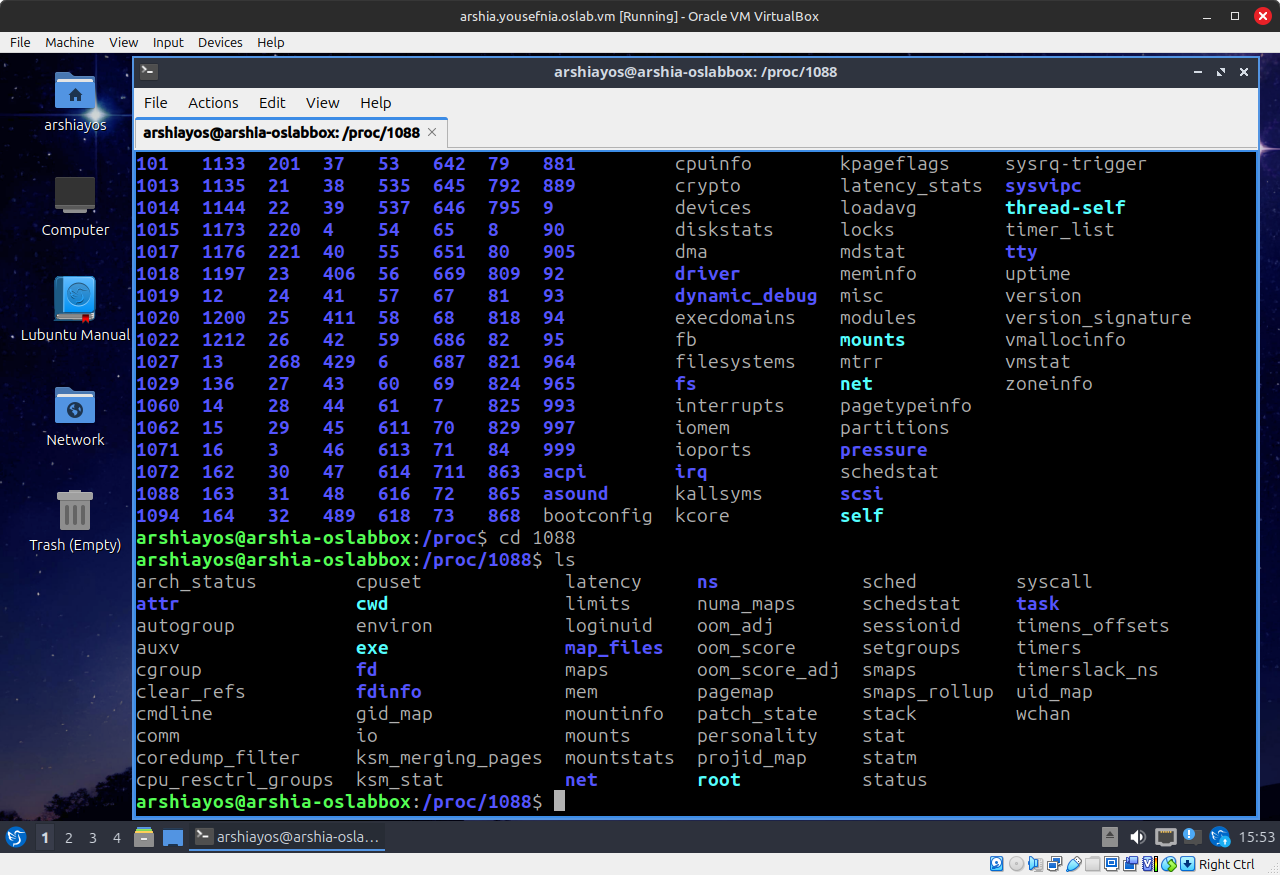
\includegraphics[width=\textwidth]{report3-resources/10.png}
		\caption{محتوای داخل یک پوشه مربوط به یک پردازه}
		\label{fig:9}
	\end{figure}
	\begin{figure}[H]
		\centering
		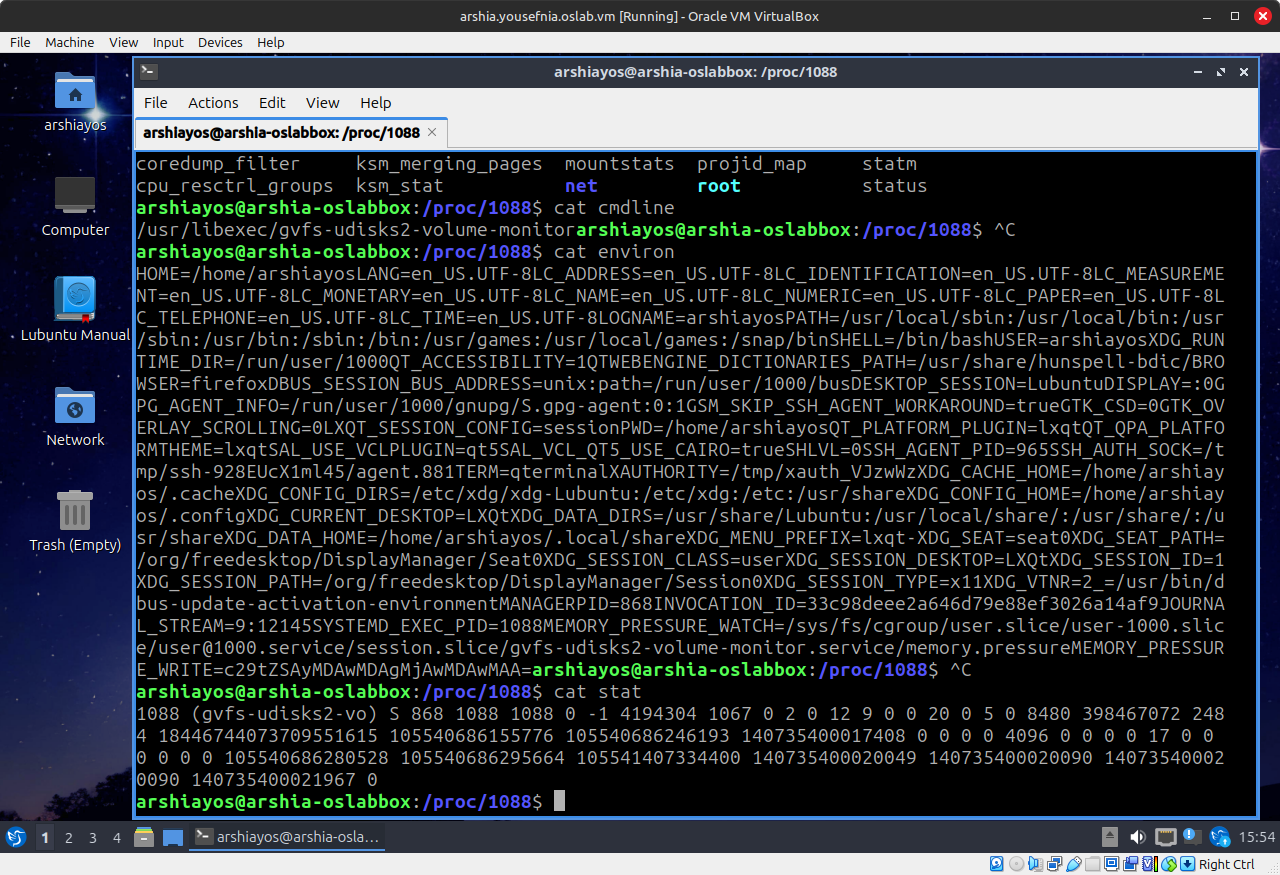
\includegraphics[width=\textwidth]{report3-resources/11.png}
		\caption{محتوای فایل‌های مختلف در پوشه پردازه}
		\label{fig:10}
	\end{figure}
	\begin{figure}[H]
		\centering
		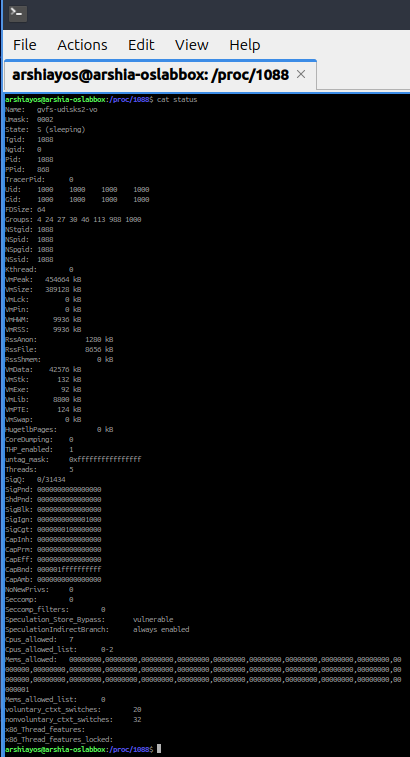
\includegraphics[width=0.7\textwidth]{report3-resources/12.png}
		\caption{محتوای فایل‌های مختلف در پوشه پردازه}
		\label{fig:11}
	\end{figure}
	\begin{figure}[H]
		\centering
		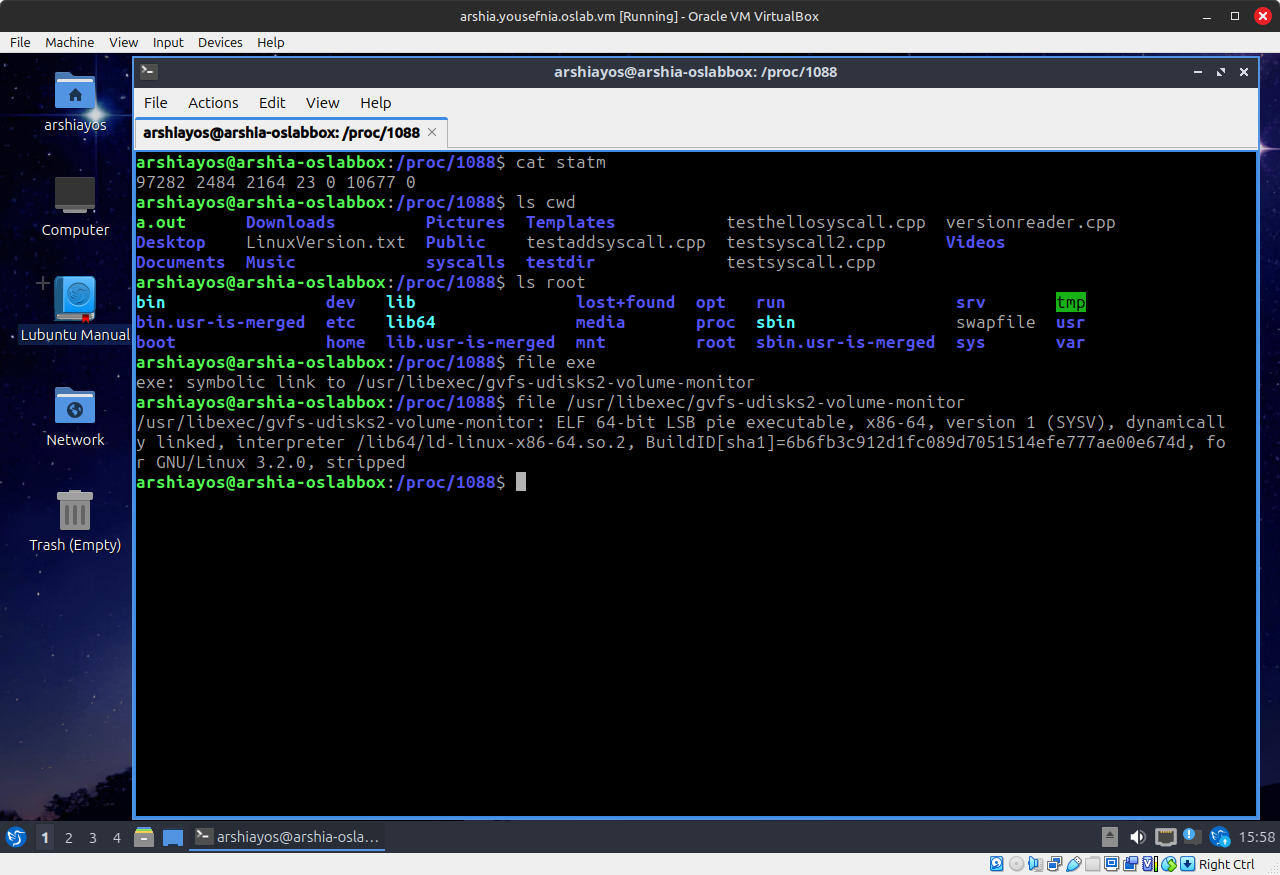
\includegraphics[width=\textwidth]{report3-resources/13.png}
		\caption{محتوای فایل‌های مختلف در پوشه پردازه}
		\label{fig:12}
	\end{figure}
	شکل \ref{fig:13} یک اسکریپت برای خواندن از مسیر /proc و خروجی دادن لیست پردازه‌ها به همراه نام آنهاست. در ادامه شکل \ref{fig:14} یک نمونه اجرای آن است.
	\begin{figure}[H]
		\centering
		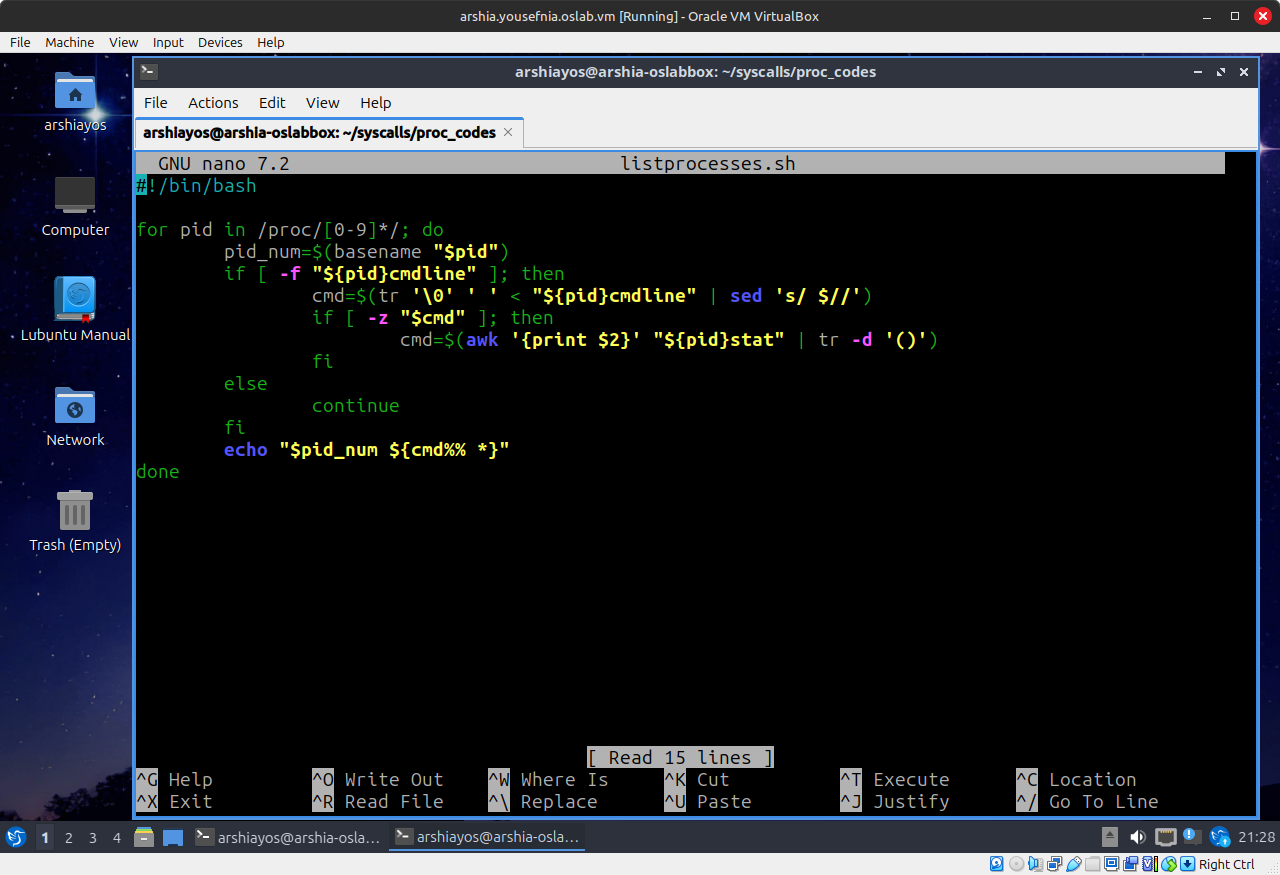
\includegraphics[width=\textwidth]{report3-resources/14.png}
		\caption{یک script برای خروجی دادن لیست شماره پردازه‌ها و نام آن‌ها}
		\label{fig:13}
	\end{figure}
	\begin{figure}[H]
		\centering
		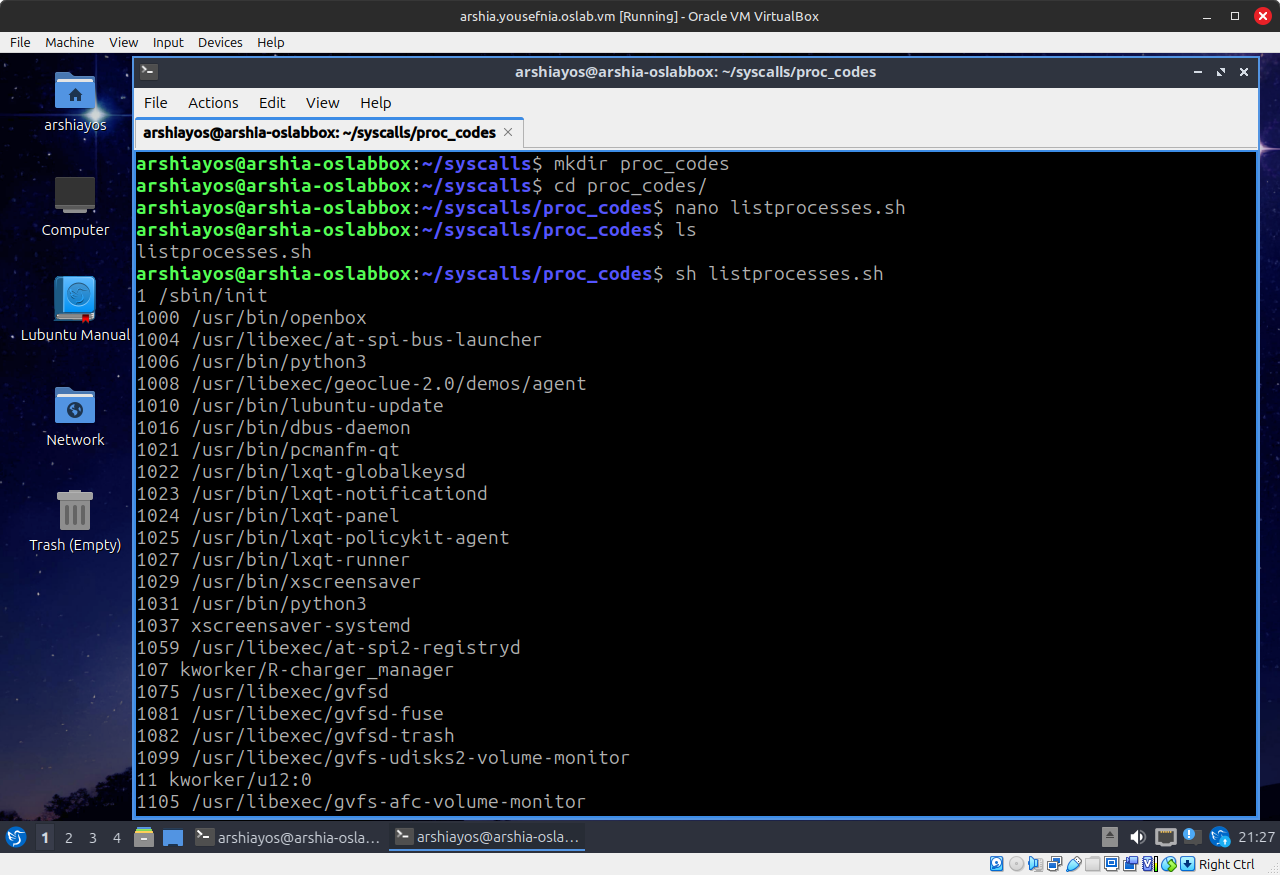
\includegraphics[width=\textwidth]{report3-resources/15.png}
		\caption{اجرای اسکریپت شکل \ref{fig:13}}
		\label{fig:14}
	\end{figure}
	
	\subsection{تمرین}
	در این تمرین یک برنامه نوشته‌ایم که شماره یک پردازه را ورودی میگیرد و ‫اطلاعاتی‬ ‫اعم‬ ‫از‬ ‫نام‬
	‫فایل‬‫اجرایی‬ ‫آن‪،‬‬ ‫مقدار‬ ‫حافظه‬ ‫مصرفی‬ ‫به‬ ‫بایت‪،‬‬ ‫پارامتر‬ ‫های‬‫اجرا‬ ‫و‬ ‫متغیرهای‬ ‫محیطی‬ ‫مربوط‬ ‫به‬ ‫آن‬ ‫در‬ ‫خروجی‬ ‫چاپ‬ می‌کند. شکل‌های ‬‬\ref{fig:15} و \ref{fig:16} کد منبع این برنامه را نشان می‌دهند. در نهایت نتیجه کامپایل و یک نمونه اجرا در شکل \ref{fig:17} آمده است.
	
	\begin{figure}[H]
		\centering
		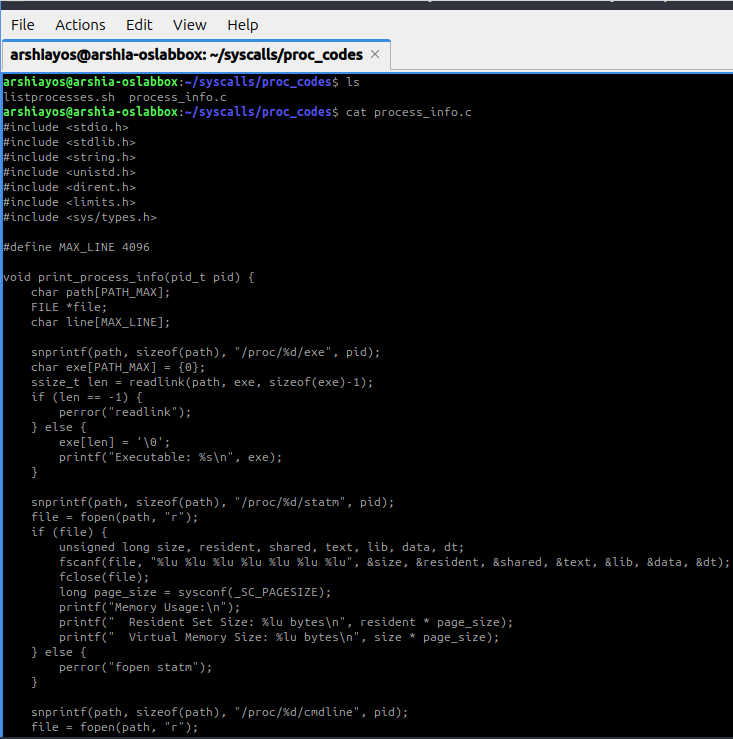
\includegraphics[width=\textwidth]{report3-resources/16.png}
		\caption{کد برنامه‌ دریافت شماره پردازه و خروجی اطلاعات مربوط به پردازه}
		\label{fig:15}
	\end{figure}
	\begin{figure}[H]
		\centering
		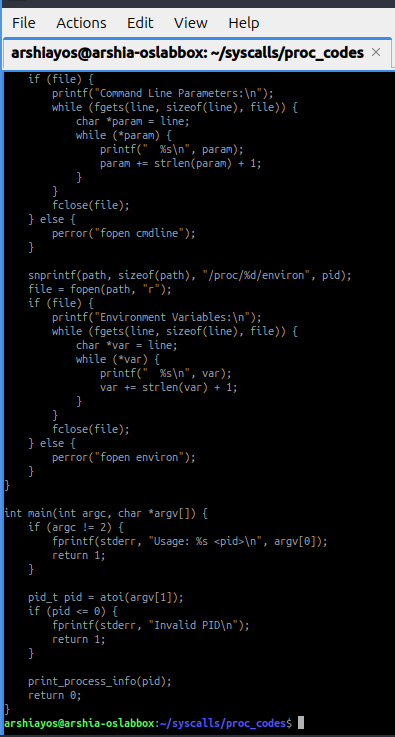
\includegraphics[width=0.8\textwidth]{report3-resources/17.png}
		\caption{ادامه کد برنامه‌ دریافت شماره پردازه و خروجی اطلاعات مربوط به پردازه}
		\label{fig:16}
	\end{figure}
	\begin{figure}[H]
		\centering
		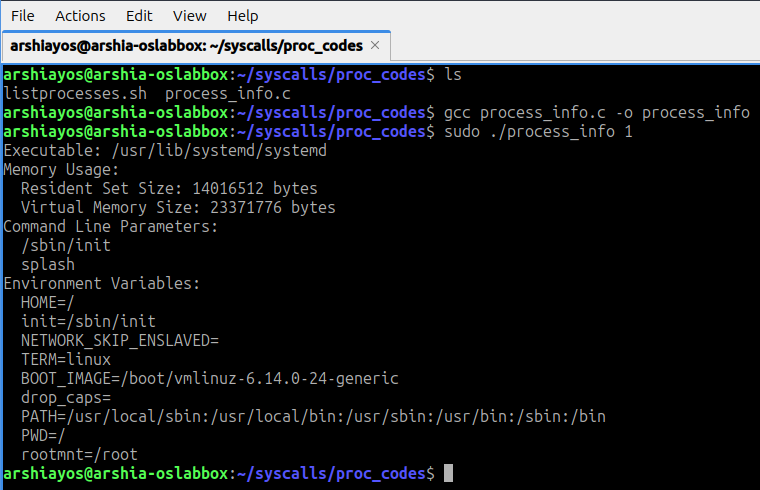
\includegraphics[width=\textwidth]{report3-resources/18.png}
		\caption{کامپایل و اجرای یک نمونه برای برنامه شکل \ref{fig:15}}
		\label{fig:17}
	\end{figure}
	
	\newpage
	\section{مشاهده اطلاعات مربوط به هسته}
	بار دیگر به به مسیر /proc می‌رویم و محتوای آن را نگاه می‌کنیم، همچنین مسیر‌های داخلی گفته شده را هم بررسی می‌کنیم تا محتوای آن‌ها را ببینیم. این موارد در شکل‌های 
	\ref{fig:18}،
	\ref{fig:19}،
	\ref{fig:20}،
	\ref{fig:21}،
	\ref{fig:22}،
	\ref{fig:23}، و
	به تفکیک آمده است.
	
	/proc/meminfo
	
	 اطلاعات مربوط به حافظه (RAM) سیستم، مانند مقدار کل، آزاد، و کش‌شده.
	
	/proc/version
	
	 نسخه هسته (Kernel) و اطلاعات مربوط به سیستم‌عامل.
	
	/proc/uptime
	
	 مدت زمانی که سیستم روشن بوده و زمان بیکار بودن \textenglish{CPU}.
	
	/proc/stat
	
	 آمارهای کلی پردازنده و فعالیت سیستم.
	
	/proc/mounts
	
	 لیست فایل‌سیستم‌های mount شده فعلی.
	
	/proc/net/
	
	 اطلاعات شبکه مانند اتصالات و آمار رابط‌های شبکه.
	
	/proc/loadavg
	
	 میانگین بار سیستم در بازه‌های زمانی مختلف.
	
	/proc/interrupts
	
	 لیست وقفه‌های سخت‌افزاری و شمارش فراخوانی‌ها.
	
	/proc/ioports
	
	 آدرس‌های ورودی/خروجی استفاده‌شده توسط سخت‌افزار.
	
	/proc/filesystems
	
	 فایل‌سیستم‌های پشتیبانی‌شده توسط هسته.
	
	/proc/cpuinfo
	
	 اطلاعات دقیق درباره پردازنده‌ها (تعداد، مدل، سرعت و غیره).
	
	/proc/cmdline
	
	 پارامترهای استفاده‌شده برای راه‌اندازی هسته هنگام بوت.
	
	\begin{figure}[H]
		\centering
		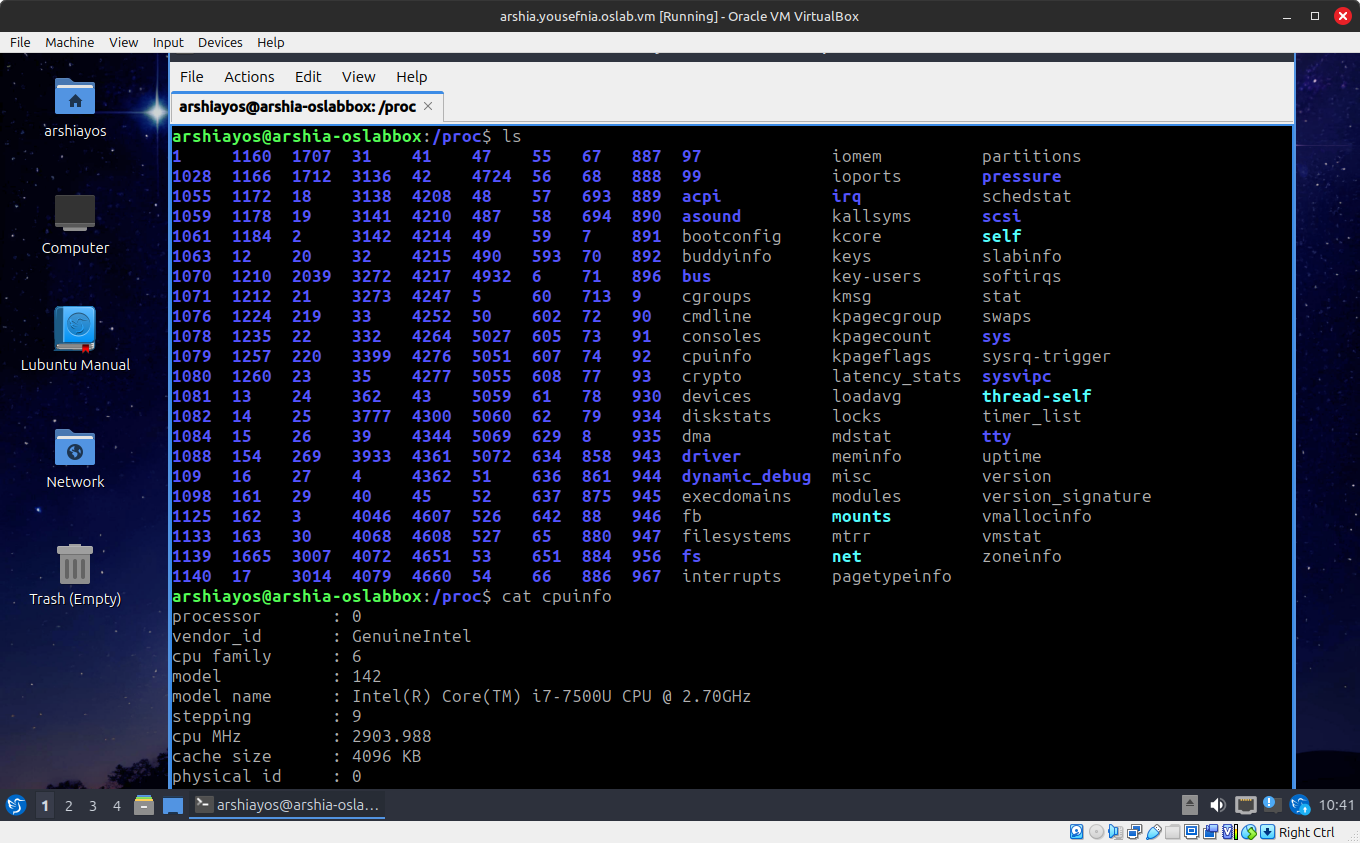
\includegraphics[width=\textwidth]{report3-resources/19.png}
		\caption{چاپ محتوای مسیر /proc و /proc/cpuinfo}
		\label{fig:18}
	\end{figure}
	\begin{figure}[H]
		\centering
		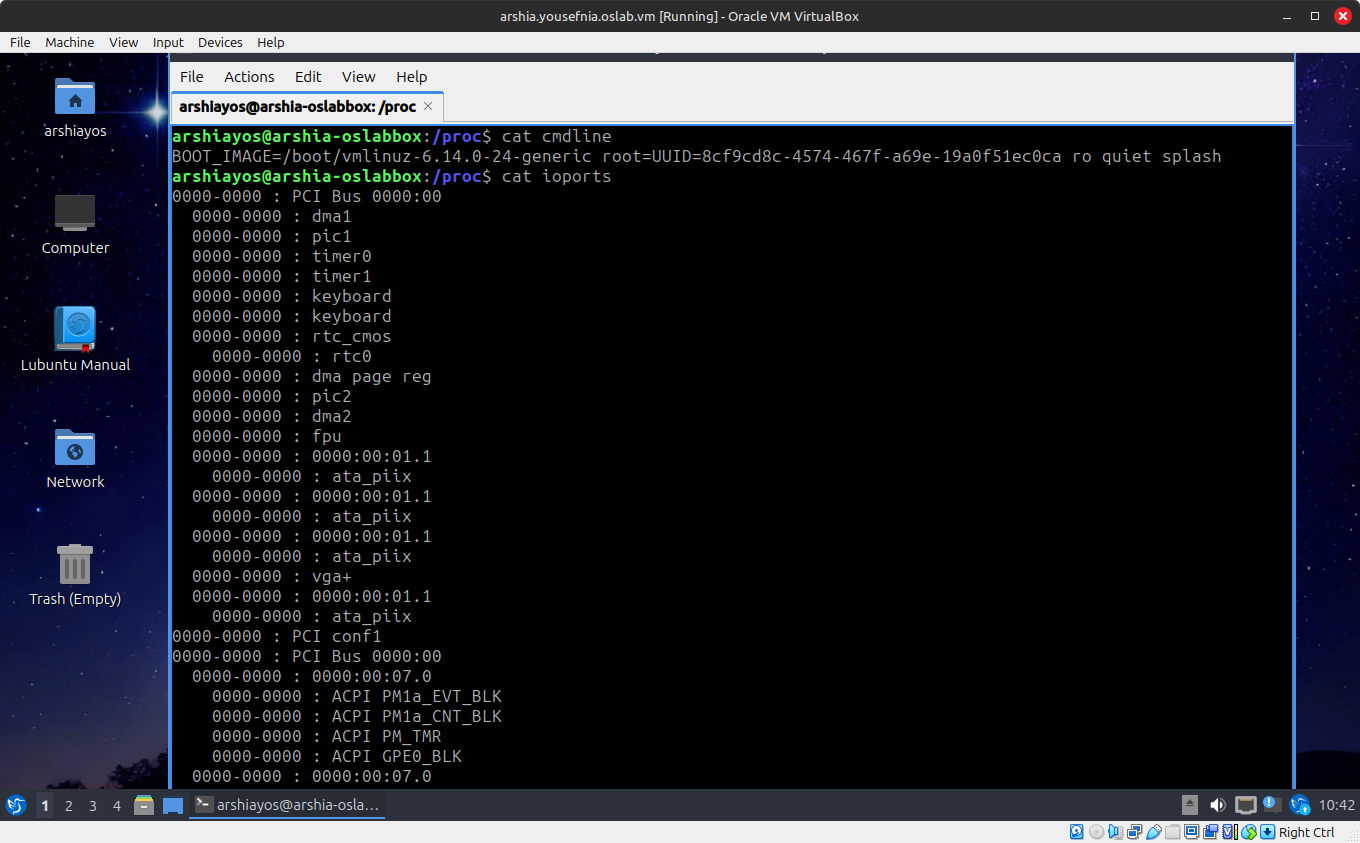
\includegraphics[width=\textwidth]{report3-resources/20.png}
		\caption{چاپ محتوای /proc/cmdline و /proc/ioports}
		\label{fig:19}
	\end{figure}
	\begin{figure}[H]
		\centering
		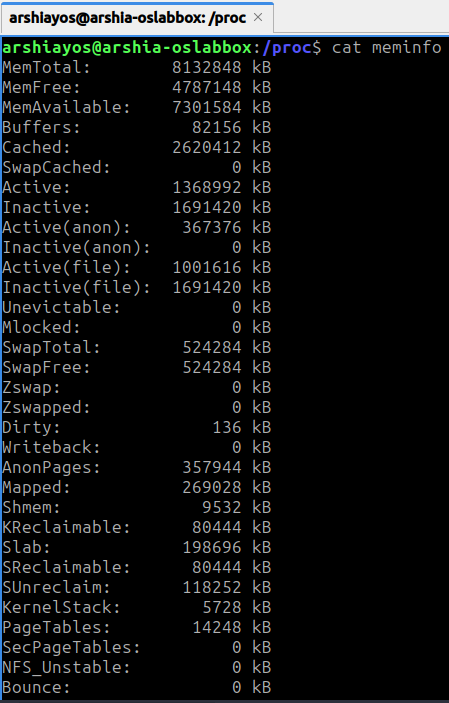
\includegraphics[width=\textwidth]{report3-resources/21.png}
		\caption{چاپ محتوای /proc/meminfo}
		\label{fig:20}
	\end{figure}
	\begin{figure}[H]
		\centering
		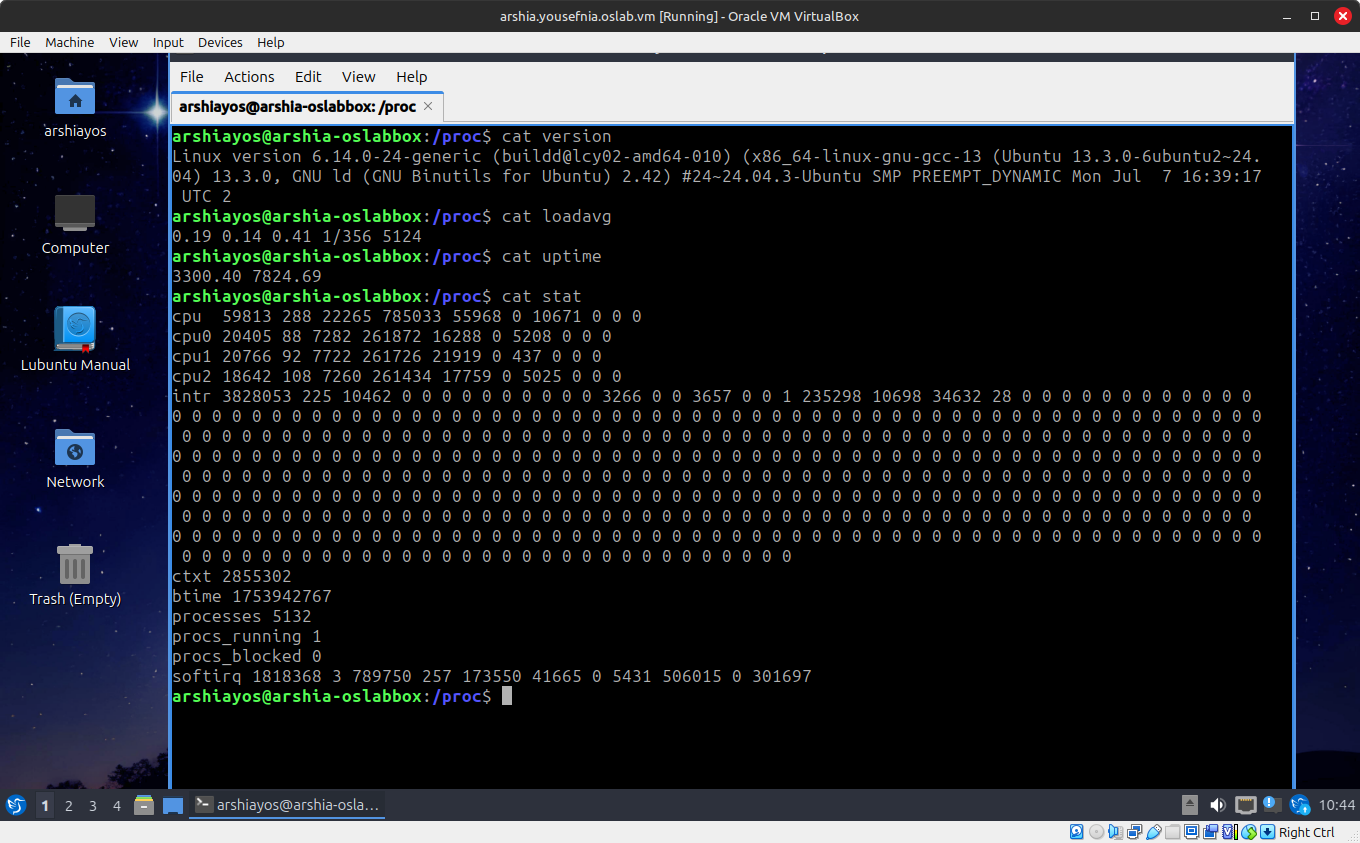
\includegraphics[width=\textwidth]{report3-resources/211.png}
		\caption{چاپ محتوای /proc/version و /proc/loadavg و /proc/uptime و /proc/stat}
		\label{fig:21}
	\end{figure}
	\begin{figure}[H]
		\centering
		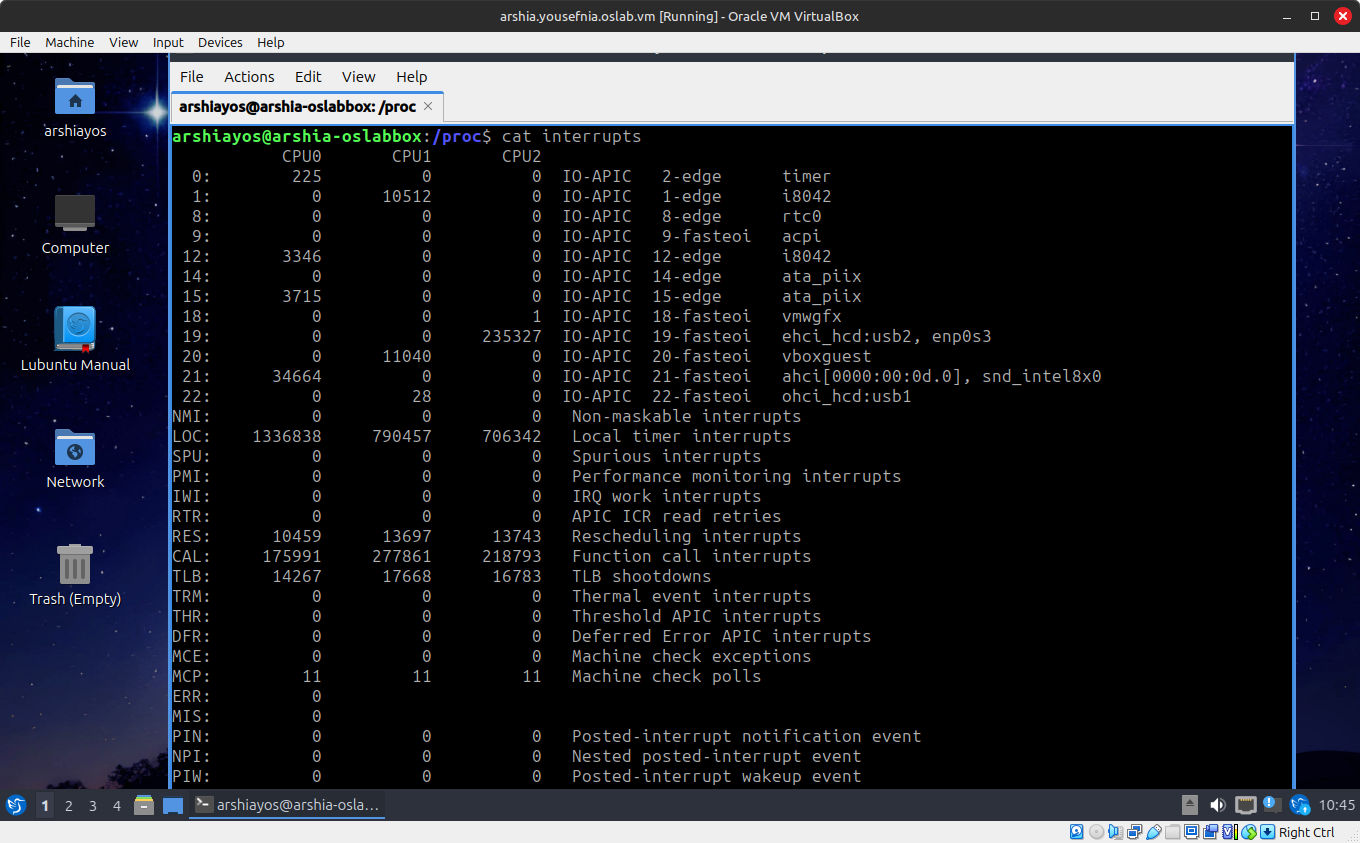
\includegraphics[width=\textwidth]{report3-resources/212.png}
		\caption{چاپ محتوای /proc/interrupts}
		\label{fig:22}
	\end{figure}
	\begin{figure}[H]
		\centering
		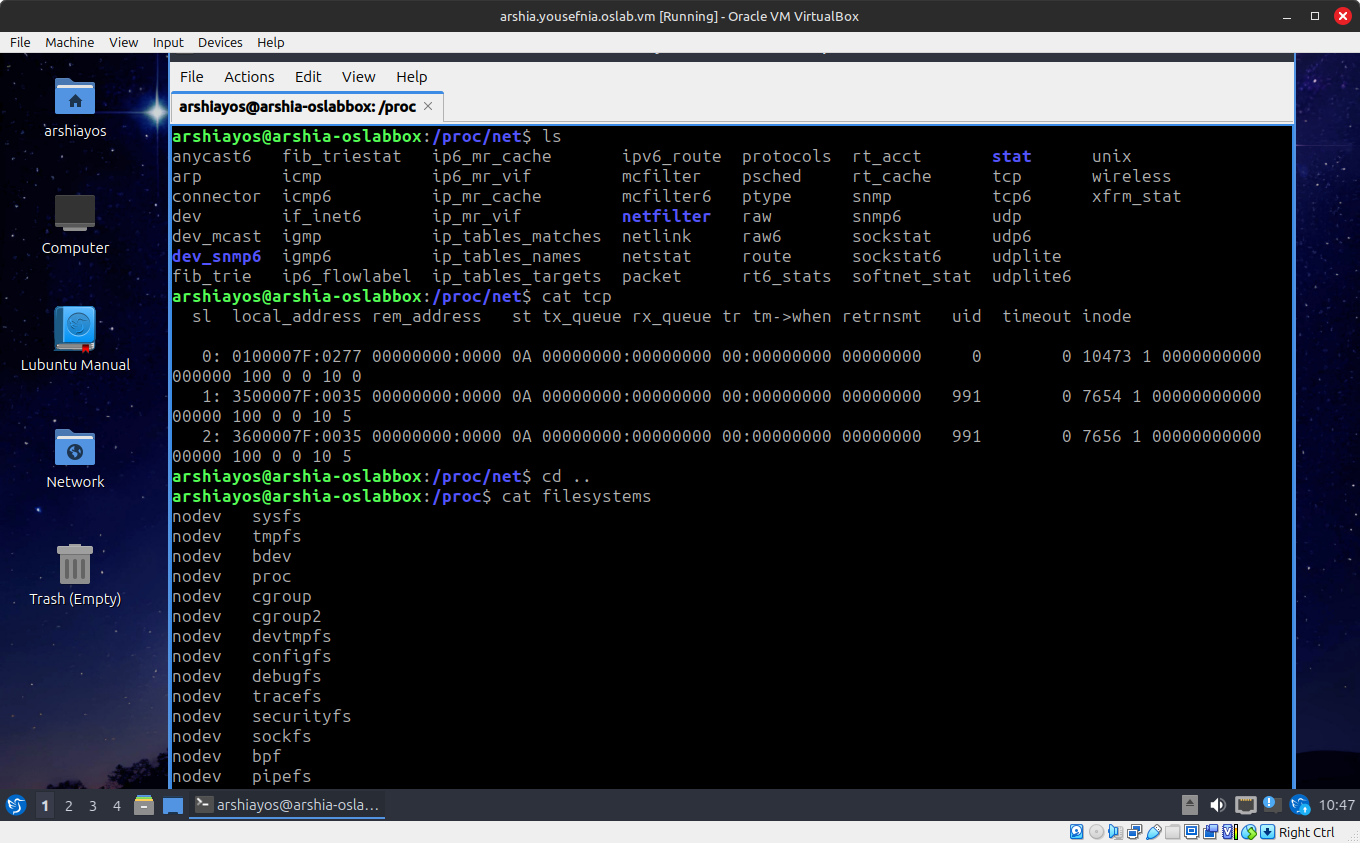
\includegraphics[width=\textwidth]{report3-resources/213.png}
		\caption{چاپ محتوای /proc/net/ و /proc/filesystems}
		\label{fig:23}
	\end{figure}
	
	در ادامه یک برنامه می‌نویسیم که ‫نام‬ ‫مدل‬ ‫پردازنده‪،‬‬ ‫فرکانس‬ ‫آن‬ ‫و‬ ‫مقدار‬ ‫حافظه‬ ‫نهان‬ ‫آن‬ ‫را‬ چاپ کنی. شکل \ref{fig:24} این کد را نشان می‌دهد و شکل \ref{fig:25} هم کامپایل و اجرای آن را نشان می‌دهد.
	\begin{figure}[H]
		\centering
		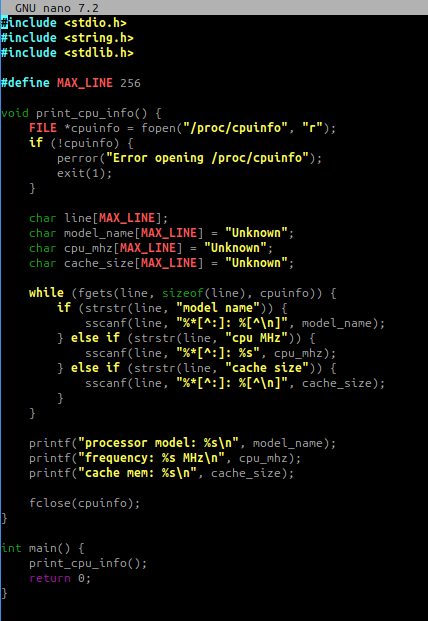
\includegraphics[width=\textwidth]{report3-resources/22.png}
		\caption{برنامه چاپ مدل و مشخصات پردازنده}
		\label{fig:24}
	\end{figure}
	\begin{figure}[H]
		\centering
		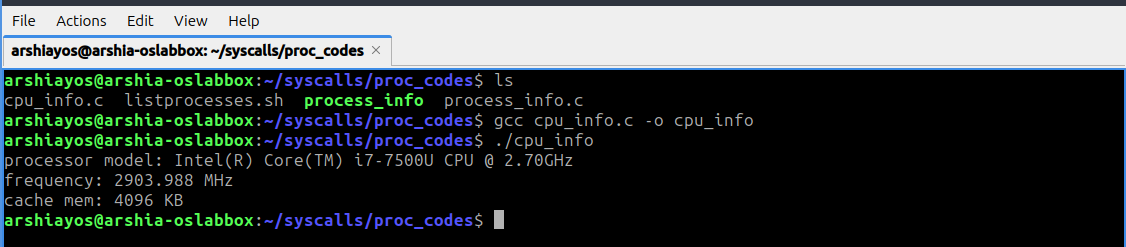
\includegraphics[width=\textwidth]{report3-resources/23.png}
		\caption{کامپایل و اجرای برنامه شکل \ref{fig:24}}
		\label{fig:25}
	\end{figure}
	
	در قسمت بعد یک برنامه دیگر می‌نویسیم که ‫مقدار‬ ‫حافظه‬ ‫کل‪،‬‬ ‫حافظه‬ ‫استفاده‬ ‫شده‬ ‫و‬ ‫حافظه‬ ‫آزاد‬ ‫را‬ ‫در‬ ‫خروجی‬ ‫چاپ‬ ‫کند‬. شکل \ref{fig:26} این کد را نشان می‌دهد و شکل \ref{fig:27} هم کامپایل و اجرای آن را نشان می‌دهد.
	\begin{figure}[H]
		\centering
		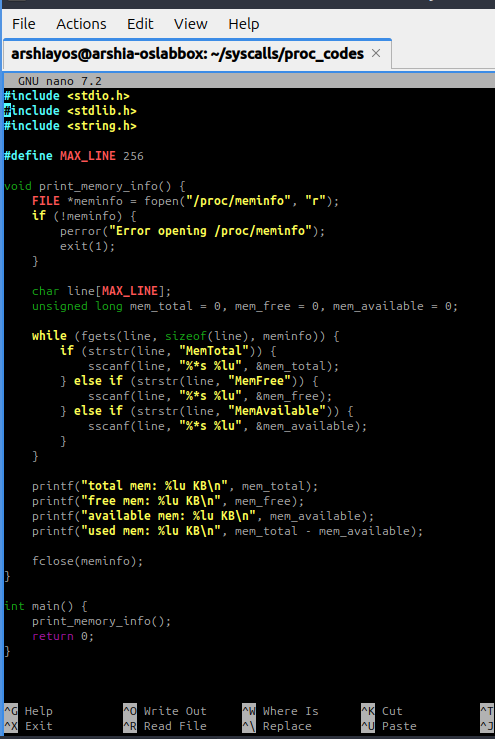
\includegraphics[width=\textwidth]{report3-resources/24.png}
		\caption{برنامه چاپ وضعیت حافظه}
		\label{fig:26}
	\end{figure}
	\begin{figure}[H]
		\centering
		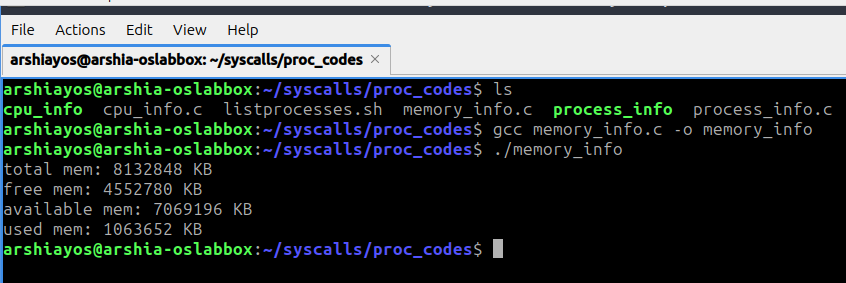
\includegraphics[width=\textwidth]{report3-resources/25.png}
		\caption{کامپایل و اجرای برنامه شکل \ref{fig:26}}
		\label{fig:27}
	\end{figure}
	
	\subsection{تمرین}
	پنج فایل مهم در /proc/sys/kernel و کاربرد آن‌ها:
	
	\subsubsection*{hostname}
	
	کاربرد: نام میزبان (Hostname) سیستم را نگه می‌دارد یا نمایش می‌دهد. این نام شناسه‌ی سیستم در شبکه است.
	
	مثال: تغییر محتوی این فایل، نام میزبان را تغییر می‌دهد.
	
	\subsubsection*{osrelease}
	
	کاربرد: نسخه کرنل لینوکس که در حال اجراست را نشان می‌دهد.
	
	مثال: بررسی ورژن کرنل برای عیب‌یابی یا مدیریت سیستم.
	
	\subsubsection*{panic}
	
	کاربرد: مشخص می‌کند سیستم پس از مواجهه با خطای بحرانی \textenglish{(kernel panic)} چه مدت صبر کند تا ریبوت شود. مقدار عددی این فایل نشان‌دهنده تعداد ثانیه‌ها است.
	
	مثال: تنظیم این مقدار برای خودکار ریبوت کردن سیستم پس از کرش.
	
	\subsubsection*{printk}
	
	کاربرد: سطح اولویت پیام‌های کرنل را تعیین می‌کند که چه پیام‌هایی باید در لاگ نمایش داده شوند.
	
	مثال: برای کنترل میزان اطلاعات گزارش شده توسط کرنل، مثلاً برای دیباگ.
	
	\subsubsection*{version}
	
	کاربرد: اطلاعات کامل‌تری درباره نسخه کرنل، شامل شماره نسخه، تاریخ کامپایل و اطلاعات بیشتر.
	
	مثال: استفاده برای تشخیص دقیق نسخه کرنل و اطلاعات مربوط به کامپایل.
	
	منبع: \cite{a1}
	
	\subsubsection*{/proc/self}
	
	در مورد /proc/self و کاربرد آن:
	/proc/self یک لینک نمادین \textenglish{(symbolic link)} است که به شاخه‌ی مربوط به فرآیند (process) ای که در حال دسترسی به این مسیر است اشاره می‌کند.
	
	یعنی اگر فرآیندی /proc/self را باز کند، در واقع به /proc/[PID] خودش اشاره دارد، یعنی شناسه فرآیند خود را نشان می‌دهد.
	
	کاربرد: این مسیر به برنامه‌ها و اسکریپت‌ها اجازه می‌دهد بدون نیاز به دانستن PID خود، اطلاعات مرتبط با فرآیند خود را بخوانند یا دستکاری کنند.
	
	مثال:
	
	/proc/self/status اطلاعات وضعیت فرآیند جاری را نشان می‌دهد.
	
	/proc/self/fd لیست توصیفگرهای فایل \textenglish{(file descriptors)} باز فرآیند جاری است.
	
	منبع: \cite{a2}
	
	

	
	% ==============================
	% References
	% ==============================
	\newpage
	\begin{LTR}
		\printbibliography[title={مراجع}]
	\end{LTR}

	
\end{document}

